\documentclass[11pt,letterpaper]{article}
\usepackage[margin=1in]{geometry}
\usepackage[T1]{fontenc}
\usepackage{amsmath,amssymb,amsthm,booktabs,array,graphicx,float}
\usepackage[nopatch={eqnum,footnote}]{microtype}
\usepackage{setspace}
\usepackage[numbers,square,sort&compress]{natbib}
\usepackage[hidelinks]{hyperref}
\usepackage{lineno}
\usepackage[font=small,labelfont=bf,labelsep=period,justification=raggedright,singlelinecheck=off]{caption}
\usepackage{fancyhdr}
\pagestyle{fancy}
\fancyhf{}
\fancyfoot[C]{\thepage}
\renewcommand{\headrulewidth}{0pt}
\newcommand{\E}{\mathbb E}
\newcommand{\R}{\mathbb R}
\newcommand{\norm}[1]{\left\lVert#1\right\rVert}
\newtheorem{proposition}{Example}
\setlength{\emergencystretch}{2em}
\setlength{\parindent}{0pt}
\setlength{\parskip}{0.4em}
\widowpenalty=10000
\clubpenalty=10000
\raggedright
\doublespacing
\hypersetup{pdftitle={Repeatable interaction scores do not guarantee a correct circuit},pdfauthor={Ihor Kendiukhov}}
\begin{document}
\linenumbers
{\Large\textbf{Repeatable interaction scores do not guarantee a correct circuit}}

\bigskip
Ihor Kendiukhov\textsuperscript{1*}

\textbf{1} Institute of Medical Genetics and Applied Genomics, University of Tübingen, Tübingen, Germany

* Correspondence: \href{mailto:ihor.kendiukhov@student.uni-tuebingen.de}{ihor.kendiukhov@student.uni-tuebingen.de}

ORCID: \href{https://orcid.org/0000-0001-5342-1499}{0000-0001-5342-1499}

\textbf{Article type:} Article

\textbf{Keywords:} mechanistic interpretability; neural networks; activation patching; circuit discovery; transformers; reproducibility
\clearpage
\section*{Abstract}
Researchers study neural networks by copying outputs of internal parts between
runs. Changing two parts together reveals when their effects do not simply
add. Can strong, repeatable interactions reveal direct connections or a small
set of parts that preserves a computation? We test GPT-2 Small and small transformers with known
task circuits. In GPT-2, 48 of 432 pairs capture 93.8\% of measured interaction
strength on new prompts, but selecting parts by individual effects reproduces
the tested block interactions better. Multiplying fitted scores for individual
parts summarizes most tables. In one known-circuit model, the ten strongest
pairs contain five direct links and five pairs connected through intermediate
parts. Three further models give closely repeated rankings, yet two assign
about 44--54\% of total score to pairs with no path in the known task circuit.
In a separate test, we kept a small connection set unchanged and replaced the
rest with values from another run; only one of three models met every criterion.
These results distinguish finding promising parts from explaining their
connections or preserving their computation. Researchers building or pruning
circuits should test these claims separately: a short, repeatable interaction
map is not enough to establish a correct circuit.


\section*{Introduction}
A model can contain thousands of parts, while a particular task may use only
a small number of them. Researchers try to find these parts and their
connections: the task's \emph{circuit}. The goal is an explanation small enough
to understand that still accounts for how the model produces its answer
\cite{conmy2023acdc,hanna2024faithfulness,kramar2024atp}.

One way to investigate a part is to copy its internal output from a run on one
input into a run on another input. If the answer changes, the copied state
has affected the computation. This procedure is often called activation
patching. Testing two parts together can reveal an effect that testing either
part alone misses. For example, one part may compensate when another is changed
\cite{vaidyanathan2026mediators,gong2026coax}.

For each pair, we compare the effect of changing both parts with the sum of
their separate effects. We collect these differences in a table, called an
interaction map. A promising map would be dominated by a few pairs, and the
same pairs would stand out on new inputs. Our initial experiments asked
whether such a map could help identify a small circuit.

This requires four separate checks. Do the scores repeat on new inputs? Does
testing pairs tell us more than testing individual parts? Do strong pairs
correspond to direct connections? When we keep a selected set of connections,
does the model still compute the answer? A pair can pass one check and fail
another. In particular, replacing two parts changes everything that happens
after them; it does not isolate the connection between them.

We study a pretrained language model and small transformers with known task
circuits. The models use attention and feed-forward components from the
Transformer architecture \cite{vaswani2017attention}; the pretrained model
is GPT-2 \cite{radford2019language}. GPT-2 provides a test in a model trained on language. The small
models let us compare scores with known direct connections and longer paths.
The experiments were designed in stages, using earlier results to choose later
tests. We use new inputs within each test, but the stages are not independent
replications of one fixed experiment.

Our contribution is to measure how these four checks can disagree. We retain
failed tests and identify the narrower findings that survive them. The study
does not assume that existing pair-intervention methods claim to recover direct
wiring; it tests whether that stronger interpretation is justified in our data. Simple examples show why an interaction need not be a direct link (Fig.~\ref{fig:counterexample}).

\subsection*{Related work}
\subsubsection*{Finding model parts and connections.}
Automated circuit discovery (ACDC) removes connections and measures the effect
\cite{conmy2023acdc}. Edge attribution patching uses a local approximation
to estimate connection importance \cite{syed2024attributionpatching}; its
integrated-gradients variant, EAP-IG, and AtP* address accuracy and cost in
different ways \cite{hanna2024faithfulness,kramar2024atp}.
These methods motivate comparisons against simpler importance scores. Our
experiments do not establish a better circuit-discovery algorithm.

Detailed studies have examined indirect object identification (IOI), a
name-completion task \cite{wang2023ioi}; copying patterns associated with
induction heads \cite{olsson2022induction}; modular arithmetic
\cite{nanda2023grokking}; numerical comparisons \cite{hanna2023greaterthan};
and factual associations \cite{meng2022rome}. These studies ask specific
questions about computations. They do not imply that an arbitrary table of
pair interactions is a model's wiring diagram.

\subsubsection*{What an internal intervention tests.}
Causal models distinguish deliberately changing a variable from observing
its value \cite{pearl2009causality}. Causal abstraction asks whether a
simpler description agrees with a neural network under specified, matched
interventions \cite{geiger2021causalabstractions,geiger2025causalabstraction}.
Distributed alignment search can find alignments with distributed neural
representations \cite{geiger2024distributedalignment}. Our pair maps do not
by themselves specify an abstract algorithm or establish such an abstraction.

Causal mediation analysis has traced contributions to language-model outputs
\cite{vig2020causalmediation}. Practical patching studies explain why the
replacement states, output measure and intervention location matter
\cite{zhang2024patchingpractices,heimersheim2024activationpatching}.
Path patching tests hypotheses about selected computational routes
\cite{goldowskydill2023pathpatching}. In contrast, replacing two parts and
recomputing everything downstream does not isolate a path between them.
Conductance assigns importance to hidden units using a different,
gradient-based construction \cite{dhamdhere2019neuron}. Intervention
libraries such as pyvene make controlled manipulations reusable
\cite{wu2024pyvene}; our experiments use separately archived code, not pyvene.

\subsubsection*{Parts can compensate for one another.}
The Hydra effect documents later computations compensating after an attention
layer is changed \cite{mcgrath2023hydra}. Work on multiple mediators and
conditional co-ablation further studies context-dependent effects and backups
\cite{vaidyanathan2026mediators,gong2026coax}. Compensation and interactions
are therefore not new findings in themselves. We ask what a repeatable pair
score establishes about direct connections and about selected parts run together.

\subsubsection*{Feature attribution and interactions.}
A separate line of work explains predictions by assigning importance to
input features. Integrated Gradients and SHAP are established examples
\cite{sundararajan2017axiomatic,lundberg2017unified}. Neural Interaction
Detection, Integrated Hessians and Archipelago examine interactions using
weights, derivatives, or changes to groups of input features
\cite{tsang2018detecting,janizek2021explaining,tsang2020archipelago}.
Their variables, reference choices and attribution rules differ from our
internal-state replacements. We do not treat their scores as direct wiring
estimates or claim to have benchmarked those methods here.

\subsubsection*{Choice of parts and evaluation.}
The Local Interaction Basis seeks representations with a small number of
important interactions \cite{bushnaq2024lib}. We instead keep the model's
existing attention heads and feed-forward blocks (multilayer perceptrons;
MLPs). A different choice of parts could produce a different map.
Tracr, InterpBench and the Mechanistic Interpretability Benchmark (MIB)
provide complementary tools for studying known computations and evaluating
interpretability methods
\cite{lindner2023tracr,gupta2024interpbench,mueller2025mib}.

Whether a selected circuit preserves behaviour is usually called
\emph{faithfulness}. Its measured value depends on what replaces the parts
outside that circuit \cite{miller2024robustness}. Such replacements can
change the computational setting and misrank candidate circuits
\cite{geng2026recovery}. Our contribution is the measured disagreement
between pair-score repeatability, simple product descriptions, direct and
indirect reference links, and joint-set tests. The general concern about
misleading circuit scores is already established.

\section*{Results}
\subsection*{A few head pairs account for most of the measured strength}
The first test, using whole blocks, failed. The 24 pairs chosen from corrected
discovery scores captured only 12.72\% of the score on new inputs. Only three
were also among the new inputs' strongest 24. Uncorrected scores did better:
61.42\% coverage and 18/24 overlap. The correction learned on the first set
did not work well on the second. This rejects that corrected-map method, not
every use of pair scores.

The closer test of individual heads gave a clearer positive result. Choosing
four heads from each block gave 48 of the 432 tested pairs. These pairs capture
93.82\% of the total interaction score on new inputs. Resampling the contexts
gives a one-sided 95\% lower bound of 92.43\%. Equally sized random choices
have only 42.64\% coverage at their 95th percentile.
Table~\ref{tab:heads} gives the results for each block pair.





The full planned test still failed. In two block pairs, fewer than 12 of 16
chosen pairs kept the same effect sign. Those sign changes occur mainly in
weak pairs, carrying only 2.83\% and 0.24\% of the selected score. The dominant
interaction strengths therefore remain repeatable despite this failure.

More importantly, choosing heads from pair scores did not improve on choosing
them from their individual effects. Pair selection was better in only one of
three block pairs. Across all three, individual-effect selection reproduced
the block interactions better: $R^2=0.9074$ versus 0.8617 for pair selection.
The pair map reveals a short, repeatable list, but this test does not show
that the list is more useful than the simpler method (Fig~\ref{fig:historical}).



\subsection*{One number per part explains most of the pair table}
After the main test, we checked whether the table needs a separate description
for each pair. It mostly does not. Multiplying one fitted number for each head
by one for its partner gives an almost complete description. On confirmation,
the best rank-one fit explains more than 99.7\% of the sum of squared table
entries. This fit statistic is different from the total score used for coverage.

Numbers fitted from discovery rows and columns predict the new pair scores
about as well as the complete old table: $R^2=0.711$ versus 0.699 across all
432 pairs. Both methods had already measured every discovery pair. The result
shows that the table is easy to summarize, not that it was cheaper to obtain.

After removing a separate rank-one fit from each table, at most 0.43\% of the
discovery table's squared norm and 0.27\% of confirmation's remains. The
remaining patterns predict the new inputs poorly: their $R^2$ is negative for
all three block pairs. Tables that keep positive and negative signs contain
some information beyond individual-head effects, but a similar product pattern
captures almost all of it. Only one small leftover pattern repeats positively,
at about 0.66\% of that table's squared norm. These checks were designed after
seeing the main results, rather than as independent confirmation tests.

\subsection*{The strongest pairs can be several steps apart}
In case 97, the pair rankings repeat almost perfectly on new inputs: their
rank correlation is 0.9973. Yet the pair scores find direct links less well
than the simple product of two fitted part scores. Average precision is
0.4899 versus 0.5370. Of the top six pairs, only two are known direct links,
compared with three for the product model. Table~\ref{tab:gt} reports every
method specified for this comparison.





Looking at the known circuit explains many of the apparent mistakes. The ten
strongest pairs contain five direct links and five pairs joined through
several steps. All ten have some connecting path. Direct links receive 41.20\%
of total score, indirect pairs 53.67\%, and the other 72 candidates 5.13\%.
The 15 pairs with any connecting path therefore hold 94.87\% of the score.
Ranking these pairs gives AP 0.8502, with 15/87 positive labels. This check
was done after seeing the main results. It shows sensitivity to longer paths
in this model, not a general method for recovering them. The highest-scoring
pair, L0 MLP--L1 MLP, has no direct link in the reference circuit.

The fitted product model explains 98.75\% of the sum of squared pair scores
and chooses the same top 15 pairs as the measured table. Removing that product
pattern does not improve the search for direct links. The positive leftover
score finds none in its top six.

\subsection*{What happens on three more models?}
All three new models repeat their pair rankings closely enough to pass the
planned test (Table~\ref{tab:fresh}). But the other patterns vary. In cases 63
and 82, the chosen 10\% of pairs capture at least 75\% of the new score, and
the product of one number per part gives a fit above 90\%. Case 103 fails
both tests. A repeatable table therefore need not be dominated by a few pairs
or have a nearly exact product description.





Case 63, our control, puts its only direct reference link first. That link
receives 98.93\% of the total score. A table dominated by one pair is easy to
fit with a product model. The result shows that pair scores can sometimes
identify a direct link very well.

In the two models with longer paths, indirectly linked pairs score much more
highly on average than pairs with no path in the reference circuit. In case
103, the means are 47.54 and 5.11. Resampling the same input pairs gives a
95\% interval of $[40.80,44.35]$ for their difference. In case 82 the means
are 69.95 and 5.06, with a difference interval of $[62.54,67.32]$. On average,
an indirect pair receives $5.45\times$ and $6.43\times$ as much score as a
uniformly chosen candidate pair in the respective models.

However, most candidate pairs have no path in the reference circuit. Despite
their lower average scores, together they receive 54.49\% and 43.71\% of the
total (Fig~\ref{fig:fresh}). These models therefore do not repeat case 97's
finding that almost all score lies on direct or indirect known connections.



Counting both direct and indirect paths gives a higher AP than counting direct
links alone: 0.7861 versus 0.6667, and 0.6998 versus 0.6186. But it also marks
more pairs as correct. Dividing AP by the fraction of positive labels reverses
that comparison: the ratios are 11.40 and 11.62 for any path, versus 19.33 and
25.67 for direct links. Higher unadjusted AP therefore does not establish that
the scores recover indirect paths better. What repeats strongly is the score
ranking, which mixes several kinds of connection.

\subsection*{Does a small selected circuit preserve the computation?}
Three later tests found useful groups of parts under the specified internal
replacements. The groups contain 8/15, 8/15, and 5/10 heads or MLPs in cases
58, 129, and 25. Keeping only candidate connections between these parts reduces
the search space to 25/87, 22/87, and 9/33 block-level links. All three groups
pass the planned tests on new inputs. Yet the selection method beats its
required comparisons in only case 129: finding a useful group does not prove
that this method finds it better than simpler alternatives.

The next experiment keeps at most 10\% of all candidate internal connections.
It chooses them on discovery inputs and runs them together on new inputs.
Only case 25 passes the full criterion (Table~\ref{tab:sets}). The other two
fail, as do the claims that all models pass the alternative-replacement and
full-input checks. This does not show that no suitable small circuit exists.
It shows that the chosen scores, selections, and budgets did not establish one
under the specified tests.





The failures have different meanings. Case 129 preserves answer loss well,
but its detailed output change scores 0.8872, below the required 0.90. In case
58, even using all connections between the shortlisted parts fails the region
check: its selected-change loss recovery is only 0.3926. The smaller choice
therefore starts from a region that already failed one requirement.

These experiments change inputs, interventions, normalization, and budgets
between stages. They do not prove that selecting parts inherently works better
than selecting connections. They show why earlier success at finding important
parts or repeatable interactions is not enough to certify a working circuit.

\section*{Discussion}
First test whether the same pairs stand out on new inputs. Then compare pair
scores with individual-part tests and with a product of one number per part.
Check direct links separately from longer paths, using known circuits or tests
that target specific connections. Finally, run the selected parts and
connections together. Each check answers a different question; repeatability
cannot replace any of the later checks.


Interaction maps can narrow the search to a manageable set of parts. That is
useful even when the map is not a wiring diagram. But researchers also use
small circuits to explain an algorithm or decide which connections can be
removed. For those purposes, confusing a repeatable score with a direct link
can produce the wrong explanation. Summarizing a block interaction is a
weaker result than showing that a small circuit still performs the task.


It may be possible to estimate one number per part from a few carefully chosen
pair tests, then test individual connections only in that smaller region.
This would need a new comparison at equal numbers of model runs: our current
fits already used the full pair table. Another option is to search for sets
by testing their combined effect, rather than adding up individual connection
scores. We have not established that either approach works better.


The language-model study uses one GPT-2 checkpoint, one name-completion task,
one background setting for the head tests, and three block pairs chosen from
earlier results. The other models are small and were chosen with knowledge of
their reference circuits. Those circuits provide a known task solution, not
proof of a unique explanation of every computation in the full model.

Copying states between runs can also create combinations the model rarely
encountered during training. Scores depend on the size of the replacement and
on later operations, including outputs approaching a limit. Squaring removes
effect signs. Tests designed after seeing earlier results are labeled, and
the intervals measure variation across inputs within each fixed model. The
evidence therefore supports conclusions about these tasks and changes, not
a universal method for reading model wiring or assuring general model behavior.



A few strong interactions can repeat on new inputs without revealing a model's
direct connections. In our tests, much of the pair table can be explained by
one number per part; some strong pairs are linked only through several steps;
and earlier success at finding useful parts does not establish that a smaller
set of connections preserves the computation. Interaction scores help guide
where to look. Direct connections and working circuits still need their own tests.

Detailed planned-test outcomes and the two targeted-connection follow-ups are provided in Supplementary Information (Supplementary Tables S1 and S2).

\section*{Methods}
\subsection*{Compare changes to one part and to two parts}
We run the model on two inputs. We then copy selected internal outputs from
the \emph{source} run into the \emph{recipient} run and let the rest of the model
recompute. For a pair of parts $i,j$, we need four runs: change neither part,
change $i$ alone, change $j$ alone, and change both. Other changes, if present,
stay fixed across all four runs. We call those fixed changes the background $B$.

Let $Y_x(S)$ be the output on recipient input $x$ after replacing the parts in
$S$ with their outputs from source input $x'$. We leave $x'$ out of this
notation for readability. For $B$ containing neither $i$ nor $j$, the
interaction is
\begin{equation}
 J_{ij}(x,x';B)=Y_x(B\cup\{i,j\})-Y_x(B\cup\{i\})
             -Y_x(B\cup\{j\})+Y_x(B).
 \label{eq:interaction}
\end{equation}
If the effects simply add, $J_{ij}=0$. A nonzero value means that the two
changes combine differently from their separate effects.

For GPT-2 IOI, $Y$ measures the change in the difference between two answer
scores, normalized by the difference between the original source and recipient
answers. For InterpBench, we keep the model's scores for all answer classes at
all positions except the special start token. At each position, we subtract
the mean score across classes. These experiments therefore measure different
outputs, under different fixed backgrounds.

To summarize the strength of a pair's interaction, we square its differences
before averaging over inputs and backgrounds:
\begin{equation}
 s_{ij}=\E_{x,x',B}\!\left[d^{-1}\norm{J_{ij}(x,x';B)}_2^2\right],
 \label{eq:energy}
\end{equation}
where $d$ is the number of output values. Squaring prevents positive and
negative differences from cancelling. We refer to $s_{ij}$ as the interaction
strength, or energy, of a pair. It does not measure information flowing through
a connection. Accounting for 94\% of this score also does not mean preserving
94\% of task performance. Additive function decompositions and variance-based
sensitivity indices provide other definitions of joint effects
\cite{hooker2004additive,sobol2001global}; our squared score has not been
made an orthogonal partition of output variance.

Eq~(\ref{eq:interaction}) gives the same value if $i$ and $j$ are exchanged.
It cannot determine which way information travels. When we draw an arrow, its
direction comes from the model's known order of computation. The two parts
could be connected directly, through several steps, or only through a later
part that uses both of their outputs.

\subsection*{Four checks that answer different questions}
\textbf{Do the scores repeat on new inputs?} We use a first set of inputs to
choose pairs, then test the same pairs on a separate set. We call these the
discovery and confirmation sets. The selected pairs' share of the confirmation
score is $\sum_{e\in S}s_e^{C}/\sum_e s_e^{C}$. A rank correlation checks whether
the same pairs tend to remain near the top.

\textbf{Do we need a separate score for every pair?} We try to predict pair
scores by multiplying one number for the first part by one number for the
second: $s_{ij}\approx a_i b_j$. We fit a separate set of numbers for each table;
the same part can receive different values in different tables or in its
earlier and later roles. This simple model is called a rank-one approximation.
For rectangular tables we use a singular value decomposition
(SVD), a classical least-squares low-rank approximation
\cite{eckart1936approximation}. When only some pairs are allowed by the order of computation, we fit
the two sets of nonnegative numbers on those pairs alone. Missing pairs are
not observations with score zero. A good fit describes the table; it does not
prove that either fitted number is a part's causal importance.

\textbf{Are the pairs direct connections?} In the small benchmark models, we
compare the scores with the known task circuit. We distinguish direct links,
pairs connected through several links, and pairs with no connecting path in
that circuit. These labels combine finer benchmark connections into links
between heads and MLPs; they do not list every physical connection in the full
transformer. Average precision (AP) summarizes whether the known links appear
near the top of a ranking. Because indirect links add more positive labels,
we also report how common each label is and how the scores are divided among
the three groups. Precision--recall comparisons depend on the positive
class and its frequency \cite{davis2006precisionrecall,saito2015precisionrecall}.
The AP/prevalence ratio reported here is a descriptive comparison, not a general
calibration that makes different retrieval tasks equivalent.

\textbf{Does the selected circuit still work?} We run changes to a selected set
and to everything outside that set. This checks what happens when the parts
are changed together. High individual scores or many correctly ranked links
do not replace this test.

\subsection*{Two simple examples}
The following examples show why strong, repeatable pair scores need not mean
direct connections. They use elementary algebra, not new theoretical results.

\begin{proposition}[Two parts feed the same output]
Suppose independent parts contribute $a_i m_i$, where $m_i$ indicates whether
part $i$ is changed. A later operation squares their sum:
$Y(m)=(\sum_i a_i m_i)^2$. With no other changes,
$J_{ij}=2a_i a_j$ and $s_{ij}=4a_i^2a_j^2$. Thus a single number for each part
predicts every pair's score, even though no part feeds another. If only a few
$a_i$ are nonzero, only a few pairs have nonzero scores.
\end{proposition}
\begin{proof}
Expand $(a_i+a_j)^2-a_i^2-a_j^2$. Squaring yields the stated score.
\end{proof}

\begin{proposition}[Information is copied along a chain]
Consider a chain that copies its input from one part to the next:
$z_1=x$, $z_{k+1}=z_k$, with output $z_n$.
The recipient input is zero and the source input is one. Replacing any $z_k$
with its source value makes the final output one. Hence
$Y(S)=\mathbf1\{S\ne\varnothing\}$. With no background changes,
every distinct pair has $J_{ij}=-1$, even if the two parts are several steps
apart. If any other part is already replaced, the pair instead has $J_{ij}=0$.
\end{proposition}
\begin{proof}
The first replaced node makes every downstream node equal to one. Thus the
four outputs for a pair are $0,1,1,1$.
\end{proof}
The first example produces a strong interaction between parts that meet only
later in the computation. The second produces one between parts linked through
several steps. A pair score alone therefore does not establish even an indirect
path; that too needs a separate check. The rank-one statement in the first
example concerns distinct parts only. Adding a zero diagonal to make a full
square table can change its rank (Fig~\ref{fig:counterexample}).




\subsection*{GPT-2 on a name-completion task}
We use one fixed GPT-2 Small model on IOI prompts, where the model must choose
the appropriate name to complete a sentence. The first experiment measured
all 253 pairs among 23 candidate attention or MLP blocks. It used 16 discovery
and 32 new confirmation contexts. We had specified a correction intended to
remove score patterns caused by answers approaching a fixed limit. The main
test asked whether a small set of corrected scores would repeat on new
inputs. It failed.

Using those earlier results, we chose three pairs of attention blocks for a
closer test: layers 5--8, 8--9, and 5--10, counting layers from zero. Each
block has 12 heads, giving 144 head pairs per block pair. We tested all of
them under four fixed backgrounds. Each background replaced ten other blocks
and left the layer-0 MLP unchanged. On 16 new discovery contexts, we chose
four heads from each block, giving 16 pairs per block pair. We then tested
those choices on 32 separate confirmation contexts. All required conditions
had to pass, including repeated effect signs and improvement over heads chosen
by their individual effects. Those two conditions failed in part of the study.

We also changed the chosen head groups together and compared the result with
changing the complete attention blocks. This was an actual group test, without
adding up pair scores or fitting an extra predictor. It checks whether the
small group reproduces the blocks' interaction, which is weaker than showing
that a pruned model still performs the full task.

\subsection*{Small models with known task circuits}
InterpBench supplies small transformers based on programs compiled by Tracr,
with known task circuits \cite{gupta2024interpbench,lindner2023tracr}. We first
used case 97, a three-layer model with four heads per layer, for a categorical
scale-by-maximum task. Its 15 heads and MLPs give 87 allowed candidate pairs.
The reference circuit, expressed in these units, has six parts and six direct
links. We tested no changes, each part alone, and every allowed pair, on 64
discovery and 128 confirmation input pairs. This required 26,592 model
examples. The pair scores failed the required improvement over simpler methods
for ranking direct links, so the follow-on cases planned within that test
were not run.

Separate follow-ups used new inputs and separately fixed plans. Cases 2 and 21
tested changes to individual directed connections after first choosing a small
set of parts. Cases 58, 129, and 25 tested small sets of parts, then small sets
of connections between them. For connection tests, the query, key, and value
inputs to attention remain separate. We knew the models and their reference
circuits when designing these tests; only the confirmation inputs were held out.

\subsection*{A further test on three models}
We next fixed a new plan before measuring interaction responses in cases 63,
103, and 82. These models count smaller sequence elements, swap adjacent
positions, and halve elements in the second half of a sequence. We already
knew their identities, reference circuits, and earlier feasibility information.
Case 63 has one direct reference link and no pairs connected only through
longer paths. It is a control for the claim that pair scores can sometimes
identify a direct link. Cases 103 and 82 contain longer paths.

We ran all three cases regardless of the first result. Each used 64 discovery
and 128 confirmation input pairs, with both inputs correctly answered by the
unchanged model. No selected input was repeated within a case. Confirmation
also excluded every candidate discovery input, including those not selected.
We saved all screening results and did not replace cases after a failure.
The models have 10, 15, and 20 parts; testing the unchanged model, single parts,
and pairs gives 44, 103, and 187 conditions. Checks across batch sizes agreed
within the fixed absolute tolerance of $10^{-4}$. The study required 84,864
model examples in 156 forward calls.

Before running, we set four tests: pair rankings must have correlation at least
0.80 across splits; the first set's top 10\% of pairs must capture at least
75\% of the new set's total score; one number per part must explain at least
90\% of the squared score-table norm; and, in the two models with longer
paths, indirectly linked pairs must have higher mean scores than pairs with
no path in the reference circuit. The rank-one fit uses the confirmation
table itself. It describes an already measured table and does not test whether
we can estimate it cheaply from discovery inputs.

For uncertainty, we bootstrap the confirmation input pairs
\cite{efron1979bootstrap}, resampling 1,000 times, and use
the 2.5th and 97.5th percentiles. These intervals describe variation across
inputs for each fixed model, not across a population of models, and are not
adjusted for multiple comparisons. The model runs and class-mean subtraction
use float32; differences and score analysis use float64.

\subsection*{Run the selected parts and connections together}
For a chosen set $S$, we ask two questions. Does changing $S$ reproduce the
effect of changing every part under study? And, if we keep $S$ unchanged while
replacing everything else, does the output stay close to the original?

Let $C$ be the original recipient output. Let $A$ be the output after replacing
every unit in the declared internal set $U$ with its source value. Let $N_S$
be the output after replacing $S$ alone, and $K_S$ the output after replacing
everything in $U$ outside $S$. We measure movement along the original-to-all-
changed difference $C-A$, and the remaining squared errors:
\begin{align}
 p_N &= \frac{\langle C-N_S,C-A\rangle}{\norm{C-A}^2}, &
 e_N &= \frac{\norm{N_S-A}^2}{\norm{C-A}^2},\\
 p_K &= \frac{\langle K_S-A,C-A\rangle}{\norm{C-A}^2}, &
 e_K &= \frac{\norm{K_S-C}^2}{\norm{C-A}^2}.
\end{align}
Here $p_N,p_K$ measure how much of the relevant output change is reproduced;
$e_N,e_K$ measure the squared error left over. We add over examples, positions,
and answer-score coordinates. We separately measure changes in cross-entropy
loss on the correct recipient answers. Values outside $[0,1]$ are retained.

Let $L_C,L_A,L_N,L_K$ be the mean cross-entropy losses on the same recipient
targets for these four outputs. The loss-recovery columns are
\begin{equation}
 \ell_N=\frac{L_N-L_C}{L_A-L_C},\qquad
 \ell_K=\frac{L_A-L_K}{L_A-L_C}.
\end{equation}
The denominator must be positive; otherwise the loss test is uninformative
and does not pass. We likewise require a positive squared output difference
for the projection and error measures.


The small-connection-set test requires at least 0.90 for both projections and
both loss-recovery measures, at most 0.10 for both squared errors, and at most
10\% of all candidate internal connections. We first check all connections
between the shortlisted parts using looser thresholds: 0.75 recovery and 0.25
error. We also test replacing outside values with their means and compare the
all-internal-change output with the actual source-input output. A later
calculation that normalizes by only the shortlisted region is reported
separately; it does not replace the original test.


\subsection*{Saved data, software and computational checks}
The original execution plans, per-input panels, saved model responses,
scoring code, and source-file hashes are described in Supplementary Information and the
accompanying archives. Supplementary Data contains numerical results and provenance;
the complete response arrays are in the repository deposit specified in the
Data Availability Statement. Supplementary Code includes the experiment and analysis
scripts, dependency records, a portable offline checker, and instructions for
obtaining third-party model artifacts. Model weights are not redistributed.
Code and documentation are at
\url{https://github.com/Biodyn-AI/sparse-interactions-maps};
the versioned data and code release is
\url{https://github.com/Biodyn-AI/sparse-interactions-maps/releases/tag/v1.0.0}.
The submission-time checking environment includes Python 3.12, PyTorch 2.13.0,
NumPy 2.5.1, and Matplotlib 3.11.1. Original acquisition records are retained
in the archives. These checking versions are not a claim that the original
runs used the same environment or that all versions give identical results. The offline
checker does not call a model or require a model download.

\subsection*{Use of artificial intelligence tools}
OpenAI Codex agents assisted with generating and revising hypotheses,
selecting and planning follow-up experiments, searching the literature,
writing and executing experimental and analysis code, inspecting saved
outputs, proposing interpretations, preparing figures, and writing and
editing the manuscript. Some workflows ran autonomously within the research
agenda and constraints set by the human author. These contributions were
substantive research assistance, not only language correction.

Numerical observations were obtained by executing programs on model runs or
saved response arrays, not by treating language-model answers as measurements.
Internal checks verified source-file hashes and input separation and
recomputed saved interaction tables and analyses. Automated critiques and
replays are internal validation, not external peer review or independent
experimental replication. They do not by themselves establish the validity
of the research questions, interpretations, or conclusions. Authorship,
scientific judgement, and accountability are not assigned to AI tools.



\subsection*{Code availability}
The experimental, analysis, plotting, and validation code is available without
access restrictions at \url{https://github.com/Biodyn-AI/sparse-interactions-maps}.
The frozen numerical-data release v1.0.0 includes the original source dependency
closure and a portable offline replay helper. Supplementary Code provides the
same code archive. Original code is MIT licensed; third-party dependencies
retain their own licenses. The present manuscript-format release is v1.2.0.
Figures were generated from recorded numerical values using Matplotlib 3.11.1
(\url{https://matplotlib.org}) and exported as native-vector graphics.

\subsection*{Ethics applicability}
These experiments use computational models and synthetic name-completion or
program-generated sequence inputs. They involve no human participants, human
samples, or animal subjects.

\section*{Data availability}
The data underlying the reported results, including original input panels, saved per-example model responses, plans, score records and metadata, are publicly available in the versioned release at \url{https://github.com/Biodyn-AI/sparse-interactions-maps/releases/tag/v1.0.0}. The complete archive is \path{Repository_Data_and_Code.zip}; its file-hash manifest and offline checker are included. Supplementary Data contains the smaller numerical-summary archive, not all response arrays. Original data are CC BY 4.0. Third-party model weights are not redistributed; their sources and revisions are identified in the repository's \path{UPSTREAM.json} and original registrations.

\bibliographystyle{naturemag}
\begin{thebibliography}{10}
\expandafter\ifx\csname url\endcsname\relax
  \def\url#1{\texttt{#1}}\fi
\expandafter\ifx\csname urlprefix\endcsname\relax\def\urlprefix{URL }\fi
\providecommand{\bibinfo}[2]{#2}
\providecommand{\eprint}[2][]{\url{#2}}

\bibitem{conmy2023acdc}
\bibinfo{author}{Conmy, A.}, \bibinfo{author}{Mavor-Parker, A.~N.},
  \bibinfo{author}{Lynch, A.}, \bibinfo{author}{Heimersheim, S.} \&
  \bibinfo{author}{Garriga-Alonso, A.}
\newblock \bibinfo{title}{Towards automated circuit discovery for mechanistic
  interpretability}.
\newblock In \emph{\bibinfo{booktitle}{Advances in Neural Information
  Processing Systems}}, vol.~\bibinfo{volume}{36},
  \bibinfo{pages}{16318--16352} (\bibinfo{year}{2023}).
\newblock
  \urlprefix\url{https://proceedings.neurips.cc/paper_files/paper/2023/hash/34e1dbe95d34d7ebaf99b9bcaeb5b2be-Abstract-Conference.html}.

\bibitem{hanna2024faithfulness}
\bibinfo{author}{Hanna, M.}, \bibinfo{author}{Pezzelle, S.} \&
  \bibinfo{author}{Belinkov, Y.}
\newblock \bibinfo{title}{Have faith in faithfulness: Going beyond circuit
  overlap when finding model mechanisms}.
\newblock In \emph{\bibinfo{booktitle}{Conference on Language Modeling}}
  (\bibinfo{year}{2024}).
\newblock \urlprefix\url{https://openreview.net/forum?id=TZ0CCGDcuT}.

\bibitem{kramar2024atp}
\bibinfo{author}{Kram{\'a}r, J.}, \bibinfo{author}{Lieberum, T.},
  \bibinfo{author}{Shah, R.} \& \bibinfo{author}{Nanda, N.}
\newblock \bibinfo{title}{{AtP*}: An efficient and scalable method for
  localizing {LLM} behaviour to components}.
\newblock \bibinfo{howpublished}{Preprint at
  \url{https://arxiv.org/abs/2403.00745}} (\bibinfo{year}{2024}).

\bibitem{vaidyanathan2026mediators}
\bibinfo{author}{Vaidyanathan, S.}, \bibinfo{author}{Arbour, D.},
  \bibinfo{author}{Mueller, A.}, \bibinfo{author}{Niekum, S.} \&
  \bibinfo{author}{Jensen, D.}
\newblock \bibinfo{title}{The curse of multiple mediators: Hidden interaction
  effects in activation patching}.
\newblock \bibinfo{howpublished}{Preprint at
  \url{https://arxiv.org/abs/2606.27510}} (\bibinfo{year}{2026}).

\bibitem{gong2026coax}
\bibinfo{author}{Gong, Z.} \emph{et~al.}
\newblock \bibinfo{title}{Conditional co-ablation: Recovering self-repair
  backups in transformer circuits}.
\newblock \bibinfo{howpublished}{Preprint at
  \url{https://arxiv.org/abs/2607.01940}} (\bibinfo{year}{2026}).

\bibitem{vaswani2017attention}
\bibinfo{author}{Vaswani, A.} \emph{et~al.}
\newblock \bibinfo{title}{Attention is all you need}.
\newblock In \emph{\bibinfo{booktitle}{Advances in Neural Information
  Processing Systems}}, vol.~\bibinfo{volume}{30} (\bibinfo{publisher}{Curran
  Associates, Inc.}, \bibinfo{year}{2017}).
\newblock
  \urlprefix\url{https://proceedings.neurips.cc/paper/2017/hash/3f5ee243547dee91fbd053c1c4a845aa-Abstract.html}.

\bibitem{radford2019language}
\bibinfo{author}{Radford, A.} \emph{et~al.}
\newblock \bibinfo{title}{Language models are unsupervised multitask learners}.
\newblock \bibinfo{type}{Tech. Rep.}, \bibinfo{institution}{OpenAI}
  (\bibinfo{year}{2019}).
\newblock
  \urlprefix\url{https://cdn.openai.com/better-language-models/language_models_are_unsupervised_multitask_learners.pdf}.

\bibitem{syed2024attributionpatching}
\bibinfo{author}{Syed, A.}, \bibinfo{author}{Rager, C.} \&
  \bibinfo{author}{Conmy, A.}
\newblock \bibinfo{title}{Attribution patching outperforms automated circuit
  discovery}.
\newblock In \emph{\bibinfo{booktitle}{Proceedings of the 7th BlackboxNLP
  Workshop: Analyzing and Interpreting Neural Networks for NLP}},
  \bibinfo{pages}{407--416} (\bibinfo{publisher}{Association for Computational
  Linguistics}, \bibinfo{year}{2024}).
\newblock \urlprefix\url{https://aclanthology.org/2024.blackboxnlp-1.25/}.

\bibitem{wang2023ioi}
\bibinfo{author}{Wang, K.}, \bibinfo{author}{Variengien, A.},
  \bibinfo{author}{Conmy, A.}, \bibinfo{author}{Shlegeris, B.} \&
  \bibinfo{author}{Steinhardt, J.}
\newblock \bibinfo{title}{Interpretability in the wild: a circuit for indirect
  object identification in {GPT-2} small}.
\newblock In \emph{\bibinfo{booktitle}{International Conference on Learning
  Representations}} (\bibinfo{year}{2023}).
\newblock \urlprefix\url{https://arxiv.org/abs/2211.00593}.

\bibitem{olsson2022induction}
\bibinfo{author}{Olsson, C.} \emph{et~al.}
\newblock \bibinfo{title}{In-context learning and induction heads}.
\newblock \bibinfo{howpublished}{Preprint at
  \url{https://arxiv.org/abs/2209.11895}} (\bibinfo{year}{2022}).

\bibitem{nanda2023grokking}
\bibinfo{author}{Nanda, N.}, \bibinfo{author}{Chan, L.},
  \bibinfo{author}{Lieberum, T.}, \bibinfo{author}{Smith, J.} \&
  \bibinfo{author}{Steinhardt, J.}
\newblock \bibinfo{title}{Progress measures for grokking via mechanistic
  interpretability}.
\newblock In \emph{\bibinfo{booktitle}{International Conference on Learning
  Representations}} (\bibinfo{year}{2023}).
\newblock \urlprefix\url{https://openreview.net/forum?id=9XFSbDPmdW}.

\bibitem{hanna2023greaterthan}
\bibinfo{author}{Hanna, M.}, \bibinfo{author}{Liu, O.} \&
  \bibinfo{author}{Variengien, A.}
\newblock \bibinfo{title}{How does {GPT-2} compute greater-than?: Interpreting
  mathematical abilities in a pre-trained language model}.
\newblock In \emph{\bibinfo{booktitle}{Advances in Neural Information
  Processing Systems}}, vol.~\bibinfo{volume}{36},
  \bibinfo{pages}{76033--76060} (\bibinfo{year}{2023}).
\newblock
  \urlprefix\url{https://proceedings.neurips.cc/paper_files/paper/2023/hash/efbba7719cc5172d175240f24be11280-Abstract-Conference.html}.

\bibitem{meng2022rome}
\bibinfo{author}{Meng, K.}, \bibinfo{author}{Bau, D.},
  \bibinfo{author}{Andonian, A.} \& \bibinfo{author}{Belinkov, Y.}
\newblock \bibinfo{title}{Locating and editing factual associations in {GPT}}.
\newblock In \emph{\bibinfo{booktitle}{Advances in Neural Information
  Processing Systems}}, vol.~\bibinfo{volume}{35},
  \bibinfo{pages}{17359--17372} (\bibinfo{year}{2022}).
\newblock
  \urlprefix\url{https://proceedings.neurips.cc/paper_files/paper/2022/hash/6f1d43d5a82a37e89b0665b33bf3a182-Abstract-Conference.html}.

\bibitem{pearl2009causality}
\bibinfo{author}{Pearl, J.}
\newblock \emph{\bibinfo{title}{Causality: Models, Reasoning, and Inference}}
  (\bibinfo{publisher}{Cambridge University Press}, \bibinfo{year}{2009}),
  \bibinfo{edition}{2nd} edn.
\newblock
  \urlprefix\url{https://www.cambridge.org/core/books/causality/B0046844FAE10CBF274D4ACBDAEB5F5B}.

\bibitem{geiger2021causalabstractions}
\bibinfo{author}{Geiger, A.}, \bibinfo{author}{Lu, H.}, \bibinfo{author}{Icard,
  T.} \& \bibinfo{author}{Potts, C.}
\newblock \bibinfo{title}{Causal abstractions of neural networks}.
\newblock In \emph{\bibinfo{booktitle}{Advances in Neural Information
  Processing Systems}}, vol.~\bibinfo{volume}{34}, \bibinfo{pages}{9574--9586}
  (\bibinfo{publisher}{Curran Associates, Inc.}, \bibinfo{year}{2021}).
\newblock
  \urlprefix\url{https://proceedings.neurips.cc/paper_files/paper/2021/hash/4f5c422f4d49a5a807eda27434231040-Abstract.html}.

\bibitem{geiger2025causalabstraction}
\bibinfo{author}{Geiger, A.} \emph{et~al.}
\newblock \bibinfo{title}{Causal abstraction: A theoretical foundation for
  mechanistic interpretability}.
\newblock \emph{\bibinfo{journal}{Journal of Machine Learning Research}}
  \textbf{\bibinfo{volume}{26}}, \bibinfo{pages}{1--64} (\bibinfo{year}{2025}).
\newblock \urlprefix\url{https://www.jmlr.org/papers/v26/23-0058.html}.

\bibitem{geiger2024distributedalignment}
\bibinfo{author}{Geiger, A.}, \bibinfo{author}{Wu, Z.}, \bibinfo{author}{Potts,
  C.}, \bibinfo{author}{Icard, T.} \& \bibinfo{author}{Goodman, N.}
\newblock \bibinfo{title}{Finding alignments between interpretable causal
  variables and distributed neural representations}.
\newblock In \emph{\bibinfo{booktitle}{Proceedings of the Third Conference on
  Causal Learning and Reasoning}}, vol. \bibinfo{volume}{236} of
  \emph{\bibinfo{series}{Proceedings of Machine Learning Research}},
  \bibinfo{pages}{160--187} (\bibinfo{publisher}{PMLR}, \bibinfo{year}{2024}).
\newblock \urlprefix\url{https://proceedings.mlr.press/v236/geiger24a.html}.

\bibitem{vig2020causalmediation}
\bibinfo{author}{Vig, J.} \emph{et~al.}
\newblock \bibinfo{title}{Investigating gender bias in language models using
  causal mediation analysis}.
\newblock In \emph{\bibinfo{booktitle}{Advances in Neural Information
  Processing Systems}}, vol.~\bibinfo{volume}{33},
  \bibinfo{pages}{12388--12401} (\bibinfo{publisher}{Curran Associates, Inc.},
  \bibinfo{year}{2020}).
\newblock
  \urlprefix\url{https://proceedings.neurips.cc/paper/2020/hash/92650b2e92217715fe312e6fa7b90d82-Abstract.html}.

\bibitem{zhang2024patchingpractices}
\bibinfo{author}{Zhang, F.} \& \bibinfo{author}{Nanda, N.}
\newblock \bibinfo{title}{Towards best practices of activation patching in
  language models: Metrics and methods}.
\newblock In \emph{\bibinfo{booktitle}{International Conference on Learning
  Representations}} (\bibinfo{year}{2024}).
\newblock
  \urlprefix\url{https://proceedings.iclr.cc/paper_files/paper/2024/file/06a52a54c8ee03cd86771136bc91eb1f-Paper-Conference.pdf}.

\bibitem{heimersheim2024activationpatching}
\bibinfo{author}{Heimersheim, S.} \& \bibinfo{author}{Nanda, N.}
\newblock \bibinfo{title}{How to use and interpret activation patching}.
\newblock \bibinfo{howpublished}{Preprint at
  \url{https://arxiv.org/abs/2404.15255}} (\bibinfo{year}{2024}).

\bibitem{goldowskydill2023pathpatching}
\bibinfo{author}{Goldowsky-Dill, N.}, \bibinfo{author}{MacLeod, C.},
  \bibinfo{author}{Sato, L.} \& \bibinfo{author}{Arora, A.}
\newblock \bibinfo{title}{Localizing model behavior with path patching}.
\newblock \bibinfo{howpublished}{Preprint at
  \url{https://arxiv.org/abs/2304.05969}} (\bibinfo{year}{2023}).

\bibitem{dhamdhere2019neuron}
\bibinfo{author}{Dhamdhere, K.}, \bibinfo{author}{Sundararajan, M.} \&
  \bibinfo{author}{Yan, Q.}
\newblock \bibinfo{title}{How important is a neuron?}
\newblock In \emph{\bibinfo{booktitle}{International Conference on Learning
  Representations}} (\bibinfo{year}{2019}).
\newblock \urlprefix\url{https://openreview.net/forum?id=SylKoo0cKm}.

\bibitem{wu2024pyvene}
\bibinfo{author}{Wu, Z.} \emph{et~al.}
\newblock \bibinfo{title}{{pyvene}: A library for understanding and improving
  {PyTorch} models via interventions}.
\newblock In \emph{\bibinfo{booktitle}{Proceedings of the 2024 Conference of
  the North American Chapter of the Association for Computational Linguistics:
  Human Language Technologies (Volume 3: System Demonstrations)}},
  \bibinfo{pages}{158--165} (\bibinfo{publisher}{Association for Computational
  Linguistics}, \bibinfo{year}{2024}).
\newblock \urlprefix\url{https://aclanthology.org/2024.naacl-demo.16/}.

\bibitem{mcgrath2023hydra}
\bibinfo{author}{McGrath, T.}, \bibinfo{author}{Rahtz, M.},
  \bibinfo{author}{Kram{\'a}r, J.}, \bibinfo{author}{Mikulik, V.} \&
  \bibinfo{author}{Legg, S.}
\newblock \bibinfo{title}{The hydra effect: Emergent self-repair in language
  model computations}.
\newblock \bibinfo{howpublished}{Preprint at
  \url{https://arxiv.org/abs/2307.15771}} (\bibinfo{year}{2023}).

\bibitem{sundararajan2017axiomatic}
\bibinfo{author}{Sundararajan, M.}, \bibinfo{author}{Taly, A.} \&
  \bibinfo{author}{Yan, Q.}
\newblock \bibinfo{title}{Axiomatic attribution for deep networks}.
\newblock In \emph{\bibinfo{booktitle}{Proceedings of the 34th International
  Conference on Machine Learning}}, vol.~\bibinfo{volume}{70} of
  \emph{\bibinfo{series}{Proceedings of Machine Learning Research}},
  \bibinfo{pages}{3319--3328} (\bibinfo{publisher}{PMLR},
  \bibinfo{year}{2017}).
\newblock
  \urlprefix\url{https://proceedings.mlr.press/v70/sundararajan17a.html}.

\bibitem{lundberg2017unified}
\bibinfo{author}{Lundberg, S.~M.} \& \bibinfo{author}{Lee, S.-I.}
\newblock \bibinfo{title}{A unified approach to interpreting model
  predictions}.
\newblock In \emph{\bibinfo{booktitle}{Advances in Neural Information
  Processing Systems}}, vol.~\bibinfo{volume}{30} (\bibinfo{publisher}{Curran
  Associates, Inc.}, \bibinfo{year}{2017}).
\newblock
  \urlprefix\url{https://proceedings.neurips.cc/paper_files/paper/2017/hash/8a20a8621978632d76c43dfd28b67767-Abstract.html}.

\bibitem{tsang2018detecting}
\bibinfo{author}{Tsang, M.}, \bibinfo{author}{Cheng, D.} \&
  \bibinfo{author}{Liu, Y.}
\newblock \bibinfo{title}{Detecting statistical interactions from neural
  network weights}.
\newblock In \emph{\bibinfo{booktitle}{International Conference on Learning
  Representations}} (\bibinfo{year}{2018}).
\newblock \urlprefix\url{https://openreview.net/forum?id=ByOfBggRZ}.

\bibitem{janizek2021explaining}
\bibinfo{author}{Janizek, J.~D.}, \bibinfo{author}{Sturmfels, P.} \&
  \bibinfo{author}{Lee, S.-I.}
\newblock \bibinfo{title}{Explaining explanations: Axiomatic feature
  interactions for deep networks}.
\newblock \emph{\bibinfo{journal}{Journal of Machine Learning Research}}
  \textbf{\bibinfo{volume}{22}}, \bibinfo{pages}{1--54} (\bibinfo{year}{2021}).
\newblock \urlprefix\url{https://www.jmlr.org/papers/v22/20-1223.html}.

\bibitem{tsang2020archipelago}
\bibinfo{author}{Tsang, M.}, \bibinfo{author}{Rambhatla, S.} \&
  \bibinfo{author}{Liu, Y.}
\newblock \bibinfo{title}{How does this interaction affect me? interpretable
  attribution for feature interactions}.
\newblock In \emph{\bibinfo{booktitle}{Advances in Neural Information
  Processing Systems}}, vol.~\bibinfo{volume}{33}, \bibinfo{pages}{6147--6159}
  (\bibinfo{publisher}{Curran Associates, Inc.}, \bibinfo{year}{2020}).
\newblock
  \urlprefix\url{https://proceedings.neurips.cc/paper_files/paper/2020/hash/443dec3062d0286986e21dc0631734c9-Abstract.html}.

\bibitem{bushnaq2024lib}
\bibinfo{author}{Bushnaq, L.} \emph{et~al.}
\newblock \bibinfo{title}{The local interaction basis: Identifying
  computationally-relevant and sparsely interacting features in neural
  networks}.
\newblock \bibinfo{howpublished}{Preprint at
  \url{https://arxiv.org/abs/2405.10928}} (\bibinfo{year}{2024}).

\bibitem{lindner2023tracr}
\bibinfo{author}{Lindner, D.} \emph{et~al.}
\newblock \bibinfo{title}{{Tracr}: Compiled transformers as a laboratory for
  interpretability}.
\newblock In \emph{\bibinfo{booktitle}{Advances in Neural Information
  Processing Systems}}, vol.~\bibinfo{volume}{36},
  \bibinfo{pages}{37876--37899} (\bibinfo{year}{2023}).
\newblock
  \urlprefix\url{https://proceedings.neurips.cc/paper_files/paper/2023/hash/771155abaae744e08576f1f3b4b7ac0d-Abstract-Conference.html}.

\bibitem{gupta2024interpbench}
\bibinfo{author}{Gupta, R.}, \bibinfo{author}{Arcuschin, I.},
  \bibinfo{author}{Kwa, T.} \& \bibinfo{author}{Garriga-Alonso, A.}
\newblock \bibinfo{title}{{InterpBench}: Semi-synthetic transformers for
  evaluating mechanistic interpretability techniques}.
\newblock In \emph{\bibinfo{booktitle}{Advances in Neural Information
  Processing Systems}}, vol.~\bibinfo{volume}{37},
  \bibinfo{pages}{92922--92951} (\bibinfo{year}{2024}).
\newblock
  \urlprefix\url{https://proceedings.neurips.cc/paper_files/paper/2024/hash/a8f7d43ae092d9a5295775eb17f3f4f7-Abstract-Datasets_and_Benchmarks_Track.html}.
\newblock \bibinfo{note}{Datasets and Benchmarks Track}.

\bibitem{mueller2025mib}
\bibinfo{author}{Mueller, A.} \emph{et~al.}
\newblock \bibinfo{title}{{MIB}: A mechanistic interpretability benchmark}.
\newblock In \emph{\bibinfo{booktitle}{Proceedings of the 42nd International
  Conference on Machine Learning}}, vol. \bibinfo{volume}{267} of
  \emph{\bibinfo{series}{Proceedings of Machine Learning Research}},
  \bibinfo{pages}{45069--45108} (\bibinfo{publisher}{PMLR},
  \bibinfo{year}{2025}).
\newblock \urlprefix\url{https://proceedings.mlr.press/v267/mueller25a.html}.

\bibitem{miller2024robustness}
\bibinfo{author}{Miller, J.}, \bibinfo{author}{Chughtai, B.} \&
  \bibinfo{author}{Saunders, W.}
\newblock \bibinfo{title}{Transformer circuit faithfulness metrics are not
  robust}.
\newblock In \emph{\bibinfo{booktitle}{Conference on Language Modeling}}
  (\bibinfo{year}{2024}).
\newblock \urlprefix\url{https://openreview.net/forum?id=zSf8PJyQb2}.

\bibitem{geng2026recovery}
\bibinfo{author}{Geng, C.} \emph{et~al.}
\newblock \bibinfo{title}{Are we recovering mechanisms? objective-level
  recovery gaps in mechanistic interpretability}.
\newblock \bibinfo{howpublished}{Preprint at
  \url{https://arxiv.org/abs/2610.02098}} (\bibinfo{year}{2026}).

\bibitem{hooker2004additive}
\bibinfo{author}{Hooker, G.}
\newblock \bibinfo{title}{Discovering additive structure in black box
  functions}.
\newblock In \emph{\bibinfo{booktitle}{Proceedings of the Tenth ACM SIGKDD
  International Conference on Knowledge Discovery and Data Mining}},
  \bibinfo{pages}{575--580} (\bibinfo{publisher}{Association for Computing
  Machinery}, \bibinfo{year}{2004}).
\newblock \urlprefix\url{https://doi.org/10.1145/1014052.1014122}.

\bibitem{sobol2001global}
\bibinfo{author}{Sobol', I.~M.}
\newblock \bibinfo{title}{Global sensitivity indices for nonlinear mathematical
  models and their {Monte Carlo} estimates}.
\newblock \emph{\bibinfo{journal}{Mathematics and Computers in Simulation}}
  \textbf{\bibinfo{volume}{55}}, \bibinfo{pages}{271--280}
  (\bibinfo{year}{2001}).
\newblock
  \urlprefix\url{https://www.sciencedirect.com/science/article/abs/pii/S0378475400002706}.

\bibitem{eckart1936approximation}
\bibinfo{author}{Eckart, C.} \& \bibinfo{author}{Young, G.}
\newblock \bibinfo{title}{The approximation of one matrix by another of lower
  rank}.
\newblock \emph{\bibinfo{journal}{Psychometrika}} \textbf{\bibinfo{volume}{1}},
  \bibinfo{pages}{211--218} (\bibinfo{year}{1936}).
\newblock \urlprefix\url{https://doi.org/10.1007/BF02288367}.

\bibitem{davis2006precisionrecall}
\bibinfo{author}{Davis, J.} \& \bibinfo{author}{Goadrich, M.}
\newblock \bibinfo{title}{The relationship between {Precision-Recall} and {ROC}
  curves}.
\newblock In \emph{\bibinfo{booktitle}{Proceedings of the 23rd International
  Conference on Machine Learning}}, \bibinfo{pages}{233--240}
  (\bibinfo{publisher}{Association for Computing Machinery},
  \bibinfo{year}{2006}).
\newblock \urlprefix\url{https://doi.org/10.1145/1143844.1143874}.

\bibitem{saito2015precisionrecall}
\bibinfo{author}{Saito, T.} \& \bibinfo{author}{Rehmsmeier, M.}
\newblock \bibinfo{title}{The {Precision-Recall} plot is more informative than
  the {ROC} plot when evaluating binary classifiers on imbalanced datasets}.
\newblock \emph{\bibinfo{journal}{PLOS ONE}} \textbf{\bibinfo{volume}{10}},
  \bibinfo{pages}{e0118432} (\bibinfo{year}{2015}).
\newblock
  \urlprefix\url{https://journals.plos.org/plosone/article?id=10.1371/journal.pone.0118432}.

\bibitem{efron1979bootstrap}
\bibinfo{author}{Efron, B.}
\newblock \bibinfo{title}{Bootstrap methods: Another look at the jackknife}.
\newblock \emph{\bibinfo{journal}{The Annals of Statistics}}
  \textbf{\bibinfo{volume}{7}}, \bibinfo{pages}{1--26} (\bibinfo{year}{1979}).
\newblock \urlprefix\url{https://doi.org/10.1214/aos/1176344552}.

\end{thebibliography}



\section*{Funding}
The author received no specific funding for this work.
\section*{Author contributions}
I.K. initiated and directed the project and set its research agenda.
Research planning, software, analyses, visualisation, and manuscript preparation
were assisted by AI agents as described in Methods. I.K. is responsible for
scientific review and final approval of the work.
\section*{Additional information}
\textbf{Competing interests.} The author has declared that no competing interests exist.

\textbf{Supplementary information.} Supplementary Information, Supplementary Data, and Supplementary Code accompany this Article.

\textbf{Correspondence.} Requests should be addressed to Ihor Kendiukhov at ihor.kendiukhov@student.uni-tuebingen.de.

\clearpage
\section*{Figure legends and figures}

\begin{figure}[H]
\centering
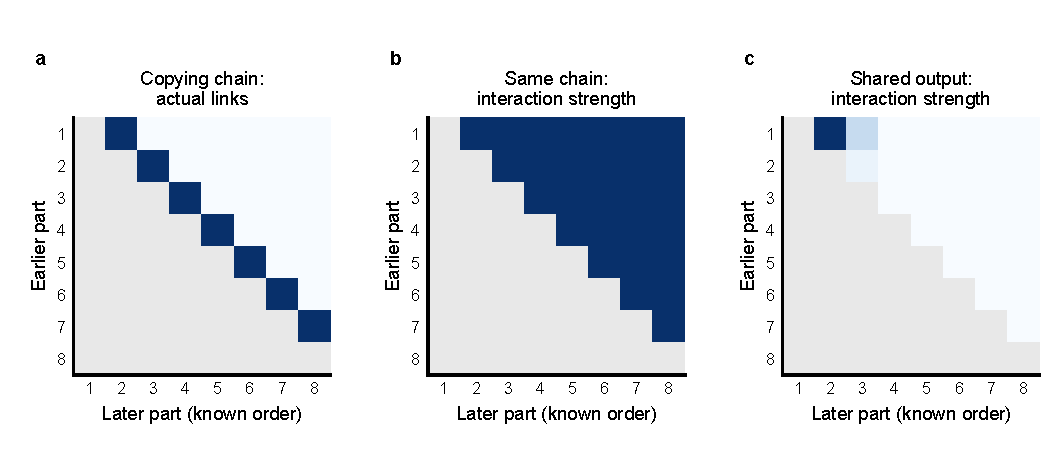
\includegraphics[width=\linewidth]{figures/Fig1.pdf}
\singlespacing
\caption{\textbf{Simple examples of misleading pair scores.} (a) A chain's actual direct links. (b) Changing pairs of parts in that chain gives a nonzero interaction for every pair, including parts several steps apart. (c) Independent parts can also interact through a later operation that squares their summed outputs. Gray cells are excluded by the known order of the parts. Blue intensity is scaled separately in each panel. Prepared with AI-assisted plotting code from recorded numerical results; no generative image model was used.}
\label{fig:counterexample}
\end{figure}

\begin{figure}[H]
\centering
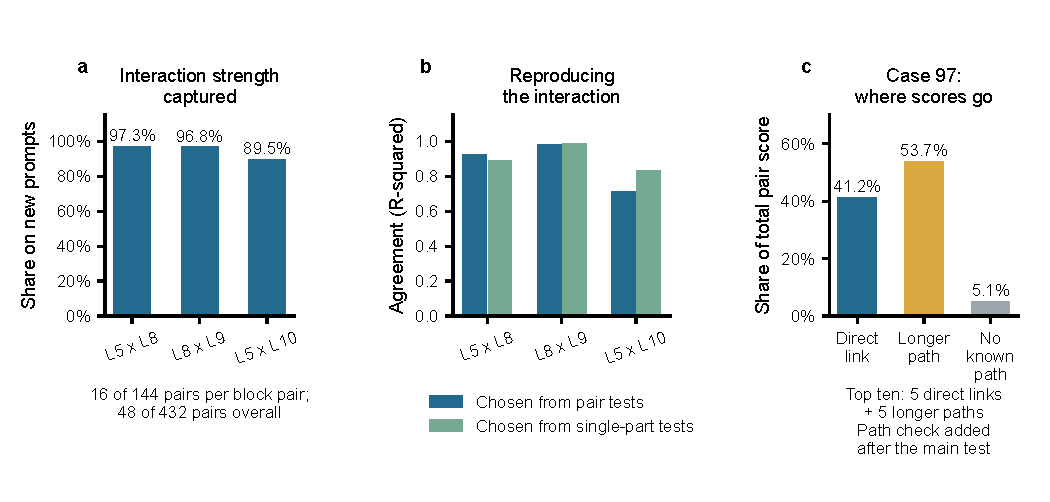
\includegraphics[width=\linewidth]{figures/Fig2.pdf}
\singlespacing
\caption{\textbf{Three results from the earlier tests.} (a) A few selected head pairs account for most interaction strength on new prompts. (b) Choosing heads from their individual effects reproduces block interactions better overall. (c) In a separate small model, most of the score belongs to direct links or pairs connected through longer paths. Matching an interaction does not by itself show that a selected circuit preserves the full task. Prepared with AI-assisted plotting code from recorded numerical results; no generative image model was used.}
\label{fig:historical}
\end{figure}

\begin{figure}[H]
\centering
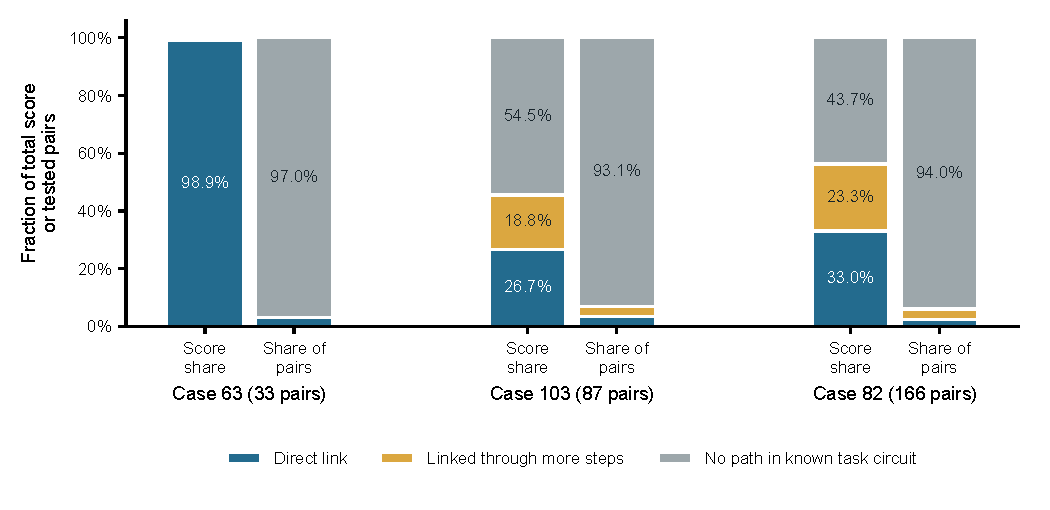
\includegraphics[width=\linewidth]{figures/Fig3.pdf}
\singlespacing
\caption{\textbf{Where the scores go in the three new models.} Each pair of bars compares the share of total score with the share of candidate pairs. Indirectly linked pairs receive high scores for their small number, but pairs with no path in the known task circuit still receive substantial total score. These labels describe the benchmark circuit; effects outside it need not be noise. Prepared with AI-assisted plotting code from recorded numerical results; no generative image model was used.}
\label{fig:fresh}
\end{figure}

\clearpage
\section*{Tables}
\begin{table}[H]
\singlespacing\centering
\caption{Results on new prompts. We select four of 12 heads from each block,
giving 16 of 144 pairs. Score share is the fraction of measured interaction
strength captured by those pairs. Group $R^2$ measures how well changing the
chosen heads together reproduces the complete blocks' interaction.}
\label{tab:heads}
\begin{tabular}{lrrrr}
\toprule
Block pair & Score share & Rank correlation & Group $R^2$ & Same sign\\
\midrule
L5A--L8A  & 0.9728 & 0.8823 & 0.9265 & 10/16\\
L8A--L9A  & 0.9681 & 0.8181 & 0.9801 & 11/16\\
L5A--L10A & 0.8947 & 0.9099 & 0.7110 & 16/16\\
\bottomrule
\end{tabular}
\end{table}

\begin{table}[H]
\singlespacing\centering
\caption{Ranking known direct links in case 97 on new inputs. Six of 87
candidates are direct links. Higher AP and receiver operating characteristic (ROC) area indicate better ranking.
AP handles equal scores together; the fixed candidate order breaks ties when
selecting the top six. Leftover scores subtract the fitted product model.}
\label{tab:gt}
\begin{tabular}{lrrr}
\toprule
Score & Average precision & ROC area & Direct links in top six\\
\midrule
Measured pair score & 0.4899 & 0.9486 & 2\\
Product of fitted part scores & 0.5370 & 0.9588 & 3\\
Product of single-part scores & 0.3922 & 0.9300 & 2\\
Absolute leftover score & 0.2485 & 0.6420 & 2\\
Positive leftover score & 0.0760 & 0.3210 & 0\\
\bottomrule
\end{tabular}
\end{table}

\begin{table}[H]
\singlespacing\centering
\caption{Three further models, each tested on 64 discovery and 128 new input
pairs. The plan was fixed before measuring interactions. ``Top 10\% share''
uses the first set's highest-scoring $\lceil0.1|E|\rceil$ pairs. Product fit
describes squared score-table error on confirmation itself, not prediction of
unseen scores. AP measures ranking of known direct links.}
\label{tab:fresh}
\begin{tabular}{lrrrrr}
\toprule
Case & Pairs tested & Rank corr. & Top 10\% share & Product fit & Direct AP\\
\midrule
63  & 33  & 0.9870 & 0.9991 & 1.0000 & 1.0000\\
103 & 87  & 0.9908 & 0.6320 & 0.8709 & 0.6667\\
82  & 166 & 0.9975 & 0.8346 & 0.9855 & 0.6186\\
\bottomrule
\end{tabular}
\end{table}

\begin{table}[H]
\singlespacing\centering\small
\caption{Run the selected connections together. Scores are normalized by
changing all internal connections under study. The $p$ columns measure output
change, and the $\ell$ columns measure loss change; $N$ changes the selected
set, while $K$ keeps it unchanged and changes the rest. The region check tests
all connections between the shortlisted parts. A full pass requires every
specified check, including squared-error and alternative-replacement tests.}
\label{tab:sets}
\begin{tabular}{lrrrrrrl}
\toprule
Case & Links kept & $p_N$ & $p_K$ & $\ell_N$ & $\ell_K$ & Region check & Full test\\
\midrule
58  & 20/207 & 0.7331 & 0.8952 & 0.2580 & 0.9982 & fail & fail\\
129 & 20/207 & 0.9987 & 0.8872 & 0.9974 & 1.0000 & pass & fail\\
25  & 7/73   & 0.9992 & 0.9545 & 0.9989 & 0.9996 & pass & pass\\
\bottomrule
\end{tabular}
\end{table}
\end{document}
